\section{Background and Related Work}
\label{sec:2}

%\begin{figure*}[h]
%    \centering
%    \includegraphics[width=1.0\textwidth]{figures/background/st_proto.png}
%    \caption{A simplified demonstration of how to define a SilverTorch model in PyTorch.}
%    \label{fig:st_prototype}
%\end{figure*}

\begin{figure}
    \centering
    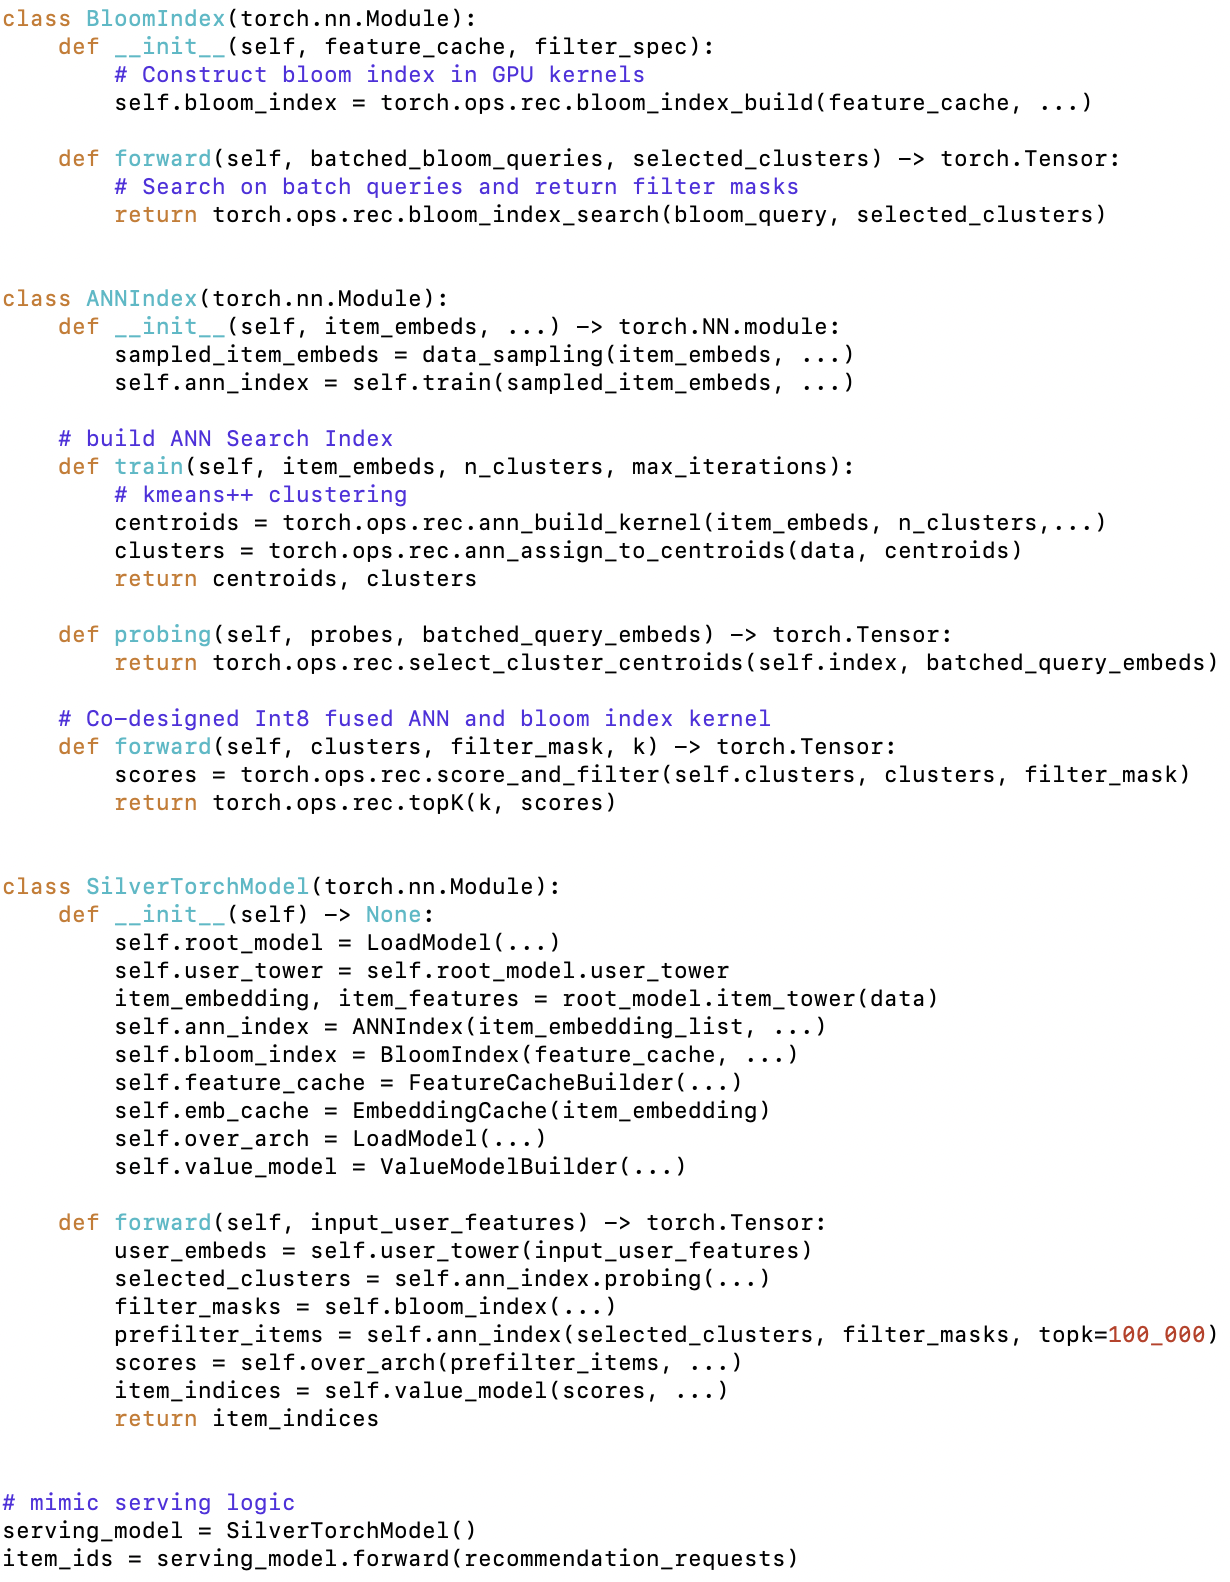
\includegraphics[width=0.5\textwidth]
    {figures/background/st_prototype.png}
    \caption{A simplified SilverTorch program in PyTorch.}
    \label{fig:st_prototype}
\end{figure}

Modern recommendation systems widely adopt the two-tower architecture~\cite{baltescu2022itemsage, covington2016deep, naumov2019deep, wang2018billion, yi2019sampling} to represent user and item features in vector space. Features for recommendation models can be categorized into dense (numerical) and sparse (categorical). User and item features contain both types, with contextual features (e.g., timestamp) bundled with user features. The embedding in our paper refers to the vector representation generated from either the user-side layers(User Tower) or the item-side layers(Item Tower). The interaction layer in retrieval is commonly simplified as dot product due to serving efficiency. The development of recommendation models primarily relies on platforms such as PyTorch~\cite{paszke2019pytorch}, TorchRec~\cite{ivchenko2022torchrec}, TensorFlow~\cite{abadi2016tensorflow}, and Jax~\cite{frostig2019compiling} which provide user-friendly Python interface for building and training neural networks. They convert models into a graph of kernel operators on GPU during execution. SilverTorch leverages PyTorch to construct all components for recommendation serving, as shown in Figure \ref{fig:st_prototype}.

%\begin{teaserfigure}
%  \includegraphics[width=\textwidth]{sampleteaser}
%  \caption{Seattle Mariners at Spring Training, 2010.}
%  \Description{Enjoying the baseball game from the third-base
%  seats. Ichiro Suzuki preparing to bat.}
%  \label{fig:st_prototype}
%\end{teaserfigure}


To efficiently retrieve items given a user embedding, a critical problem is vector search, which is a trending topic in domains like natural language processing~\cite{lewis2020retrieval}, computer vision~\cite{zhai2019learning}, search~\cite{huang2020embedding}, and recommendation systems~\cite{zhao2023embedding}. Existing solutions are either using libraries like Faiss~\cite{douze2024faiss} as dedicated services~\cite{huang2020embedding} or building a vector database~\cite{pace2025lance, wang2021milvus}. Libraries like Faiss-GPU~\cite{johnson2019billion}, Milvus~\cite{wang2021milvus} and CAGRA~\cite{ootomo2024cagra} provide GPU implementations for ANN search. Unfortunately, they only support topk and probes up to 2048~\cite{FaissGPULimitation} and topk up to 1024~\cite{MilvusGPULimitation}. As retrieval models for recommendation evolve, tens of thousands items returned from ANN search are fed into interaction layers~\cite{ding2025retrieval}. SilverTorch provides a PyTorch native implementation of nearest neighbor search running on GPUs and is highly efficient and customizable. SilverTorch's ANN module can efficiently return tens of thousands items. For feature filtering, traditional search engines~\cite{brin1998anatomy, cambazoglu2016scalability, huang2020embedding} employ inverted index which can be also applied to recommendation. These systems are CPU-based solutions and introduce overhead and cost when serving recommendation models. SilverTorch's bloom index idea is motivated by Bitfunnel~\cite{goodwin2017bitfunnel}, which tries to replace the inverted index in text search with bloom-filter-based signatures. However, Bitfunnel is a CPU solution and not specifically designed for recommendation. In recommendation, the cardinality of the feature attributes for each item is orders of magnitude smaller. 
Both the existing ANN search index and inverted index are originally designed for other applications, requiring customizations for recommendation. 
In contrast, SilverTorch's model-based approach defines the ANN search and the feature filtering within PyTorch model layers running on GPUs. The unified authoring allows us to co-design the ANN search, the feature filtering and the OverArch.

Recommendation models are becoming more complex in terms of compute, model complexity and data~\cite{ardalani2022understanding, zhang2024wukong}. Serving these models is challenging but is not well studied. SilverTorch aims to support serving evolving recommendation model architectures. ~\cite{zhai2023revisiting} extends the dot-product retrieval with the idea of mixture of logits and h-indexer, and shows the advantages using such complex structures. ~\cite{zhang2025optimizing} proposes multi-task multi-head approach for item-to-item-based retrieval. But these works do not discuss their infrastructures to serve such advanced model architectures. LiNR~\cite{borisyuk2024linr} proposes model-based retrieval on GPUs. Unlike SilverTorch, LiNR does not provide co-designed index and does not propose a GPU solution for filtering. It also does not discuss the cost efficiency of introducing GPUs. Merlin~\cite{oldridge2020merlin} discusses the possibility of using GPU to accelerate the whole stack of recommendation from data processing, training to inference, but it is a combination of different libraries using GPUs.